% stock

\newpage
À partir de ce choix d’écriture, le système suivant est défini :\\\\
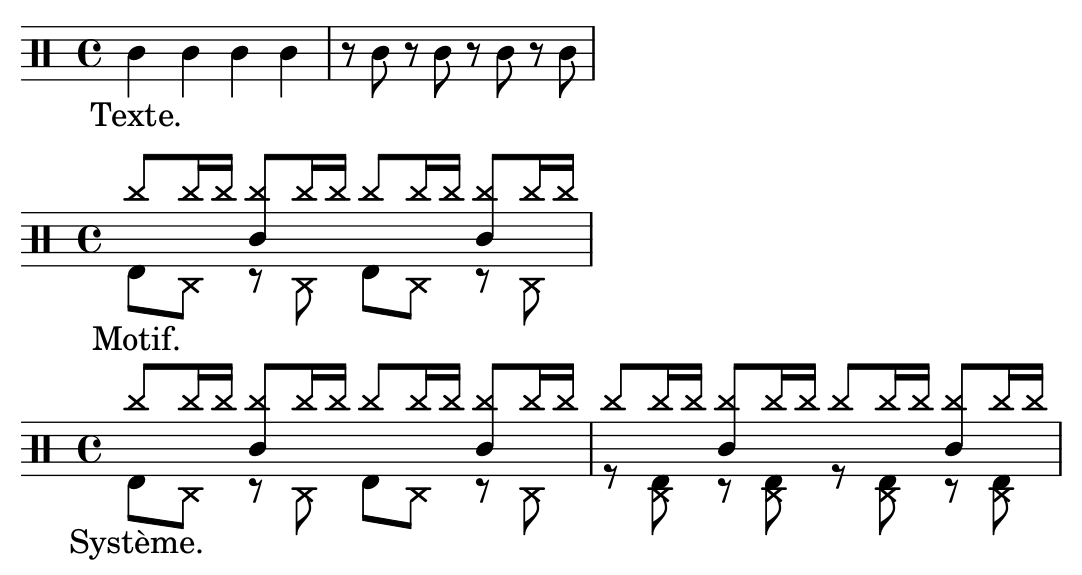
\includegraphics[height=65mm, width=115mm]{z_images/3_experimentations/system_drummer_01_session1_004.png}\\
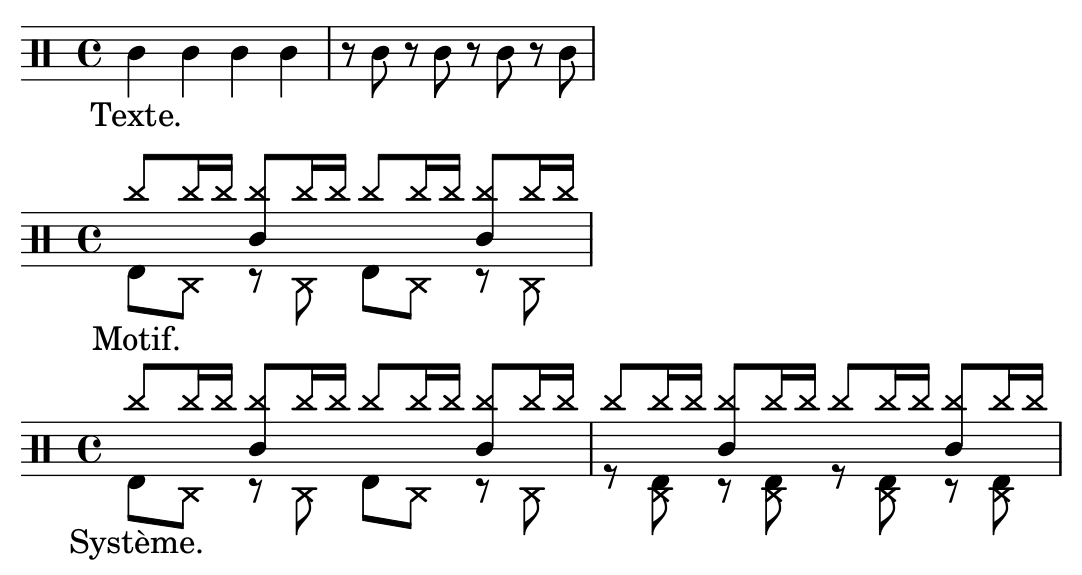
\includegraphics[height=65mm, width=115mm]{z_images/3_experimentations/system_drummer_01_session1_004.png}\\
Dans le motif, la grosse caisse est notée car elle fait partie de l’équilibre musical de ce rythme mais rigousement, elle ne devrait pas y apparaître puisque qu’elle sera indiquée par le texte.\\
Dans ce système, les noires ne doivent jamais tomber en même temps que les caisse-claires, donc, quand le texte donnera des noires sur les deuxièmes et quatrièmes temps, elles ne seront jamais jouées par le batteur (exemple sur la première mesure du système).\\


Voici la représentation de ce système en arbre de rythme :\\

\resizebox{420pt}{!}{\Tree[.Système [.Mesure\ 1  [.Temps\ 1 [51\\36 ][ [51\\44 ][51 ]]]
	[.Temps\ 2 [51\\38 ][ [51\\44 ][51 ]]]
	[.Temps\ 3 [51\\36 ][ [51\\44 ][51 ]]]
	[.Temps\ 4 [51\\38 ][ [51\\44 ][51 ]]] ]
	[.Mesure\ 2 [.Temps\ 1 [51 ][ [51\\44\\36 ][51 ]]]
	[.Temps\ 2 [51\\38 ][ [51\\44\\36 ][51 ]]]
	[.Temps\ 3 [51 ][ [51\\44\\36 ][51 ]]]
	[.Temps\ 4 [51\\38 ][ [51\\44\\36 ][51 ]]] ]]}\\

\subsubsection{Séparation des voix}
\resizebox{430pt}{!}{\Tree[.Voix\ haute 
	[.Mesure\ 1 
	[. [rd ][. [rd ][rd ]]]
	[. [rd\\cc ][. [rd ][rd ]]]
	[. [rd ][. [rd ][rd ]]]
	[. [rd\\cc ][. [rd ][rd ]]] ]
	[.Mesure\ 2 
	[. [rd ][. [rd ][rd ]]]
	[. [rd\\cc ][. [rd ][rd ]]]
	[. [rd ][. [rd ][rd ]]]
	[. [rd\\cc ][. [rd ][rd ]]] ]]}\\\\\\
\resizebox{400pt}{!}{\Tree[.Voix\ basse 
	[.Mesure\ 1 
	[. [gc ][. [pf ][tie ]]]
	[. [tie ][. [pf ][tie ]]]
	[. [gc ][. [pf ][tie ]]]
	[. [tie ][. [pf ][tie ]]] ]
	[.Mesure\ 2 
	[. [tie ][. [pf\\gc ][tie ]]]
	[. [tie ][. [pf\\gc ][tie ]]]
	[. [tie ][. [pf\\gc ][tie ]]]
	[. [tie ][. [pf\\gc ][tie ]]] ]]}

\subsubsection{Réécriture (Simplification)}
\resizebox{400pt}{!}{\Tree[.Voix\ basse 
	[.Mesure\ 1 
	[. [gc ][pf ]]
	[. [tie ][pf ]]
	[. [gc ][pf ]]
	[. [tie ][pf ]] ]
	[.Mesure\ 2 
	[. [tie ][pf\\gc ]]
	[. [tie ][pf\\gc ]]
	[. [tie ][pf\\gc ]]
	[. [tie ][pf\\gc ]] ]]}\\\\
La voix haute reste inchangée.
%preamble:
%
%
%%\usetikzlibrary{backgrounds}
%%\usetikzlibrary{trees}
%
%
%Figure 1:
%
%\begin{figure}
%\centering
%\begin{subfigure}
%[$\frac{1}{2} \frac{1}{4} \frac{1}{4}$]
%{
%\begin{tabular}{c}
%%\includegraphics[scale=\scorescale]{images/1a.png}\\
%\begin{tikzpicture} [-,thick]
%\tikzstyle{level 1}=[level distance=7mm,sibling distance=6mm]
%\tikzstyle{level 2}=[level distance=7mm,sibling distance=5mm]
%\node {$\deux$}
%  child { node {$\note$} }
%  child { node {$\deux$}
%    child { node {$\note$} }
%    child { node {$\note$} } };
%\end{tikzpicture}
%\end{tabular}
%%\label{fig:subfig1a}}
%%
%\hspace{0.6cm}
%\begin{subfigure}
%[$\lbrack \frac{1}{6} \rbrack\, \frac{1}{6}\,
%  \lbrack \frac{1}{6} \rbrack\, \frac{1}{6}\,
%  \lbrack \frac{1}{6} \rbrack\, \frac{1}{6}$]
%{
%\begin{tabular}{c}
%%\includegraphics[scale=\scorescale]{images/1b.png}\\
%\begin{tikzpicture} [-,thick]
%\tikzstyle{level 1}=[level distance=7mm,sibling distance=9mm]
%\tikzstyle{level 2}=[level distance=7mm,sibling distance=5mm]
%\node {$\trois$}
%  child { node {$\deux$}
%    child { node {$\rest$} }
%    child { node {$\note$} } }
%  child { node {$\deux$}
%    child { node {$\rest$} }
%    child { node {$\note$} } }
%  child { node {$\deux$}
%    child { node {$\rest$} }
%    child { node {$\note$} } };
%\end{tikzpicture}
%\end{tabular}
%%\label{fig:subfig1b}}
%%
%\hspace{0.6cm}
%\subfig
%[$\frac{1}{5} \frac{1}{5}
%  \frac{1}{15}\frac{1}{15}\frac{1}{15}
%  \frac{1}{5} \frac{1}{5}$]
%{
%\begin{tabular}{c}
%%\includegraphics[scale=\scorescale]{images/1c.png}\\
%\begin{tikzpicture} [-,thick]
%\tikzstyle{level 1}=[level distance=7mm,sibling distance=5mm]
%\tikzstyle{level 2}=[level distance=7mm,sibling distance=5mm]
%\node {$\cinq$}
%  child { node {$\note$} }
%  child { node {$\note$} }
%  child { node {$\trois$}
%    child { node {$\note$} }
%    child { node {$\note$} }
%    child { node {$\note$} } }
%  child { node {$\note$} }
%  child { node {$\note$} } ;
%\end{tikzpicture}
%\end{tabular}
%\label{fig:subfig1c}}
%%
%\begin{RR}
%\hspace{0.6cm}
%\subfig
%[$\frac{1}{12} \frac{1}{12} \frac{1}{12} \frac{1}{12} \frac{1}{3}
%\frac{1}{12} \frac{1}{12} \frac{1}{12} \frac{1}{12}$]
%{
%\begin{tabular}{c}
%%\includegraphics[scale=0\scorescale]{images/1d.png}\\
%%\hspace{0.3cm}
%\begin{tikzpicture} [-,thick]
%\tikzstyle{level 1}=[level distance=7mm,sibling distance=9mm]
%\tikzstyle{level 2}=[level distance=6mm,sibling distance=8mm]
%\tikzstyle{level 3}=[level distance=6mm,sibling distance=5mm]
%\node {$\trois$}
%  child { node {$\deux$}
%    child { node {$\deux$}
%      child { node {$\note$} }
%  child { node {$\note$} } }
%    child { node {$\deux$}
%      child { node {$\note$} }
%  child { node {$\note$} } } }
%  child { node {$\note$} }
%  child { node {$\deux$}
%    child { node {$\deux$}
%      child { node {$\note$} }
%  child { node {$\note$} } }
%    child { node {$\deux$}
%      child { node {$\note$} }
%  child { node {$\note$} } } };
%\end{tikzpicture}
%\end{tabular}
%\label{fig:subfig1d}}
%\end{RR}
%\caption{Simple trees of $\T(\Sigmar)$ with their corresponding
%rhythmic notations and values.}
%\label{fig:trees0}
%\end{figure}